\documentclass[main.tex]{subfiles}

\begin{document}

\chapter{The combined \gls{sd} spectrum}
\label{chapter:sd750_combined_spectrum}

In this chapter we present an update of the \sd{750} spectrum, previously published in 2021 ~\cite{PierreAuger:2021:InfillSpectrum} together with the combined \sd{433}-\sd{750} spectrum.
For the \sd{750} the efficiency measured with hybrid events and simulations from Refs. ~\cite{PierreAuger:2021:InfillSpectrum,Coleman:2020:Thesis} is revisited and parameterized in a data-driven method using the events in common with the \sd{433} in \cref{sec:sd750_response}.
An update of the dataset is presented in \cref{sec:sd750_dataset} to determine the raw spectrum.
The spectrum is then unfolded using the updated response function and unfolding in \cref{sec:sd750_spectrum}.
Finally the two spectrum measured individually with \sd{433} and the \sd{750} are combined using a likelihood method together with a study of the robustness of the measurement in \cref{sec:combined_spectrum}

\section{Updated SD-750 dataset}
\label{sec:sd750_dataset}

In 2021, the Pierre Auger Collaboration presented a measurement of a turn-down in the cosmic ray flux at around $10^{17}\,\mathrm{eV}$, consisting in about $\num{560000}$ events.
However, the feature could not be constrained due to the closeness with the minimum energy in the flux measurement, $\lg(E/\mathrm{eV})=17$.
Therefore, the width of the transition and the spectral index above the feature were fitted from the spectrum.
Given the much larger surface of the \sd{750}, energies up to $\lg(E/\mathrm{eV})=19.5$ were used in the spectrum determination.
This allowed for the ankle in the cosmic ray spectrum to be measured.

The \sd{750} started acquiring Phase I data when including the Gen II triggers, \gls{totd} and \gls{mops}, in Jan 2014 and ended with the inclusion of the new updated electronics on 29 November 2021.
The geometrical reconstruction is analogous to the one presented in \cref{subsec:geometry_ldf}.
However, in this case the reconstruction was performed using the other algorithm reconstruction, Herald, given that the Observer reconstruction was not updated for the \sd{750}.%[To do: include herald quote]
The fiducial 6T5 trigger is also applied to ensure the proper reconstruction of the events and given the inclusion of the Gen. II triggers with a strong sensitivity to the electromagnetic component of the shower, only events with $\theta<40^\circ$ are included in the spectrum measurement.
Time periods with acquisition problems are also excluded in the spectrum.
When removing the bad periods and using the number of hexagons, analogously to the \sd{433}, the exposure of the \sd{750} can be calculated, obtaining $\exposuresym_{\text{SD-750}}=$\SDSevenFiftyExposure above the full efficiency threshold.

\subsection{\sd{750} Efficiency}
\label{subsec:sd750_efficiency}

The \sd{750} efficiency was previously estimated using the limited hybrid dataset from events in common with Cohiueco and from simulations ~\cite{2018:Coleman:Thesis}.
Since the \sd{433} is nested within the \sd{750}, opens the possibility to estimate the efficiency from the events in common between the two detectors.
Having in mind that  there is the caveat that the two energy scales are interwined, hoewever we can study the efficiency since the most important contribution to this study is the full efficiency threshold.
The parameterization for the efficiency can also be estimated from this study but the contribution in the spectrum is solely in the forward-folding and hence is minor.
Using the events when both detectors were active in phase I, the binned efficiency of the \sd{750} can be estimated as 
\begin{align}
    \varepsilon(E_i)=\frac{k_i}{n_i},
\end{align}
\noindent where $n_i$ is the number of events in the $i$-eth bin detected by the \sd{433} and $k_i$ is the number of events detected in common by the \sd{750}.
The estimation was performed, as with the calibration, from the unique id tag of the events and double checked with the GPS time.
In \cref{fig:sd750_efficiency}, the circle data points represent the estimated efficiency of the \sd{750} together with the $68\%$ Clopper-Pearson confidence intervals in the error bars ~\cite{Clopper:1934:BinomialInverval}.
The efficiency results is shown for energies above the full efficiency threshold of the \sd{433}.

\begin{figure}
    \centering
    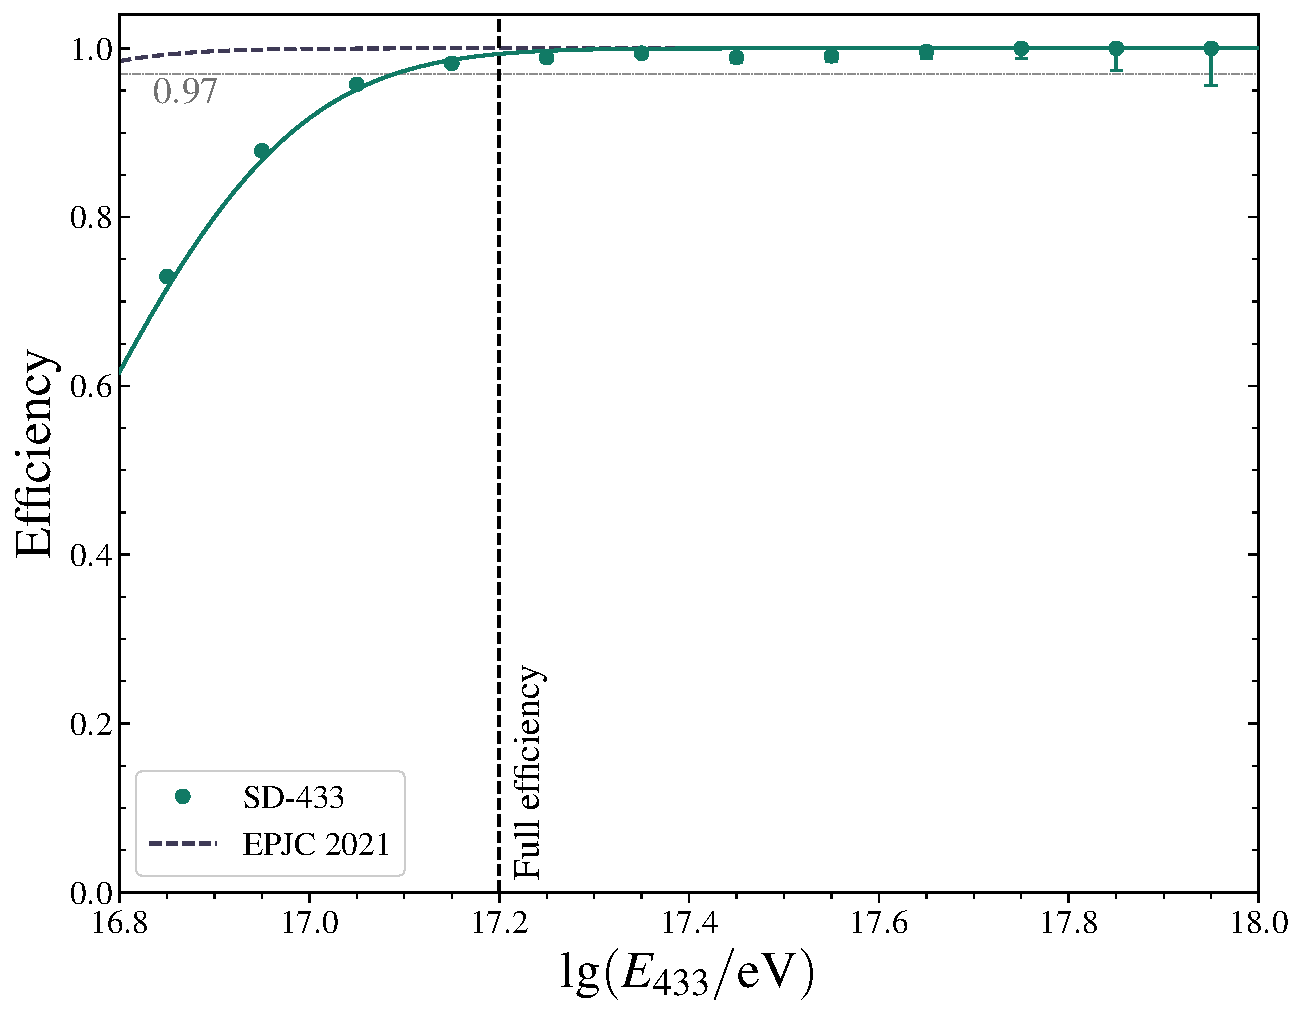
\includegraphics[width=0.8\linewidth]{figures/chapter_combined/sd750_efficiency.pdf}
    \caption{Reconstruction efficiency of the \sd{750} as a function of the energy reconstructed with the \sd{433}. The filled markers show the efficiency obtained with the updated dataset, while the open markers show the efficiency reported in the previous \sd{750} spectrum measurement~\cite{PierreAuger:2021:InfillSpectrum}. The horizontal dashed line indicates an efficiency of $0.97$.}
    \label{fig:sd750_efficiency}
\end{figure}
This confidence intervals were used to ensure that for $\varepsilon=1$, the confidence interval reduces to a lower limit, compatible with the physical constrain of the efficiency.
To parameterize the efficiency, a binomial likelihood fit was used where for each bin,
\begin{align}
    \mathcal{L}(\mu,\sigma)=\prod\limits_i^{N_{bins}}\binom{n_i}{k_i}\varepsilon_i^{k_i}(1-\varepsilon_i)^{n_i-k_i}.
\end{align}
The efficiency is modelled using the same parameterization from Ref.~\cite{PierreAuger:2021:InfillSpectrum},
\begin{align}
    \varepsilon = \frac{1}{2}\left[
1+\mathrm{erf}\left(\frac{lg(E/\mathrm{eV)-\mu}}{\sigma}\right)
    \right]
\end{align}
\noindent where $\mathrm{erf}(E)$ is the error function and $\mu$ and $\sigma$ are the shape parameters that govern the transition.
The best fit parameters are $\mu=16.74\pm0.01$ and $\sigma=(0.250\pm0.001)$ with a correlation $\rho_{\mu,\sigma}=0.38$.
The fit result is shown with a solid line in \cref{fig:sd750_efficiency}, together with the fit result from Ref.~\cite{PierreAuger:2021:InfillSpectrum} in a dashed line.
The gray vertical line shows the full efficiency threshold for the \sd{750} estimated with the \sd{433}.
It is noteworthy that the resolution previously estimated reaches full efficiency almost two bins below this work.

\subsection{Detector response}
\label{sec:sd750_response}

In order to construct the migration matrix of the \sd{750}, the resolution and bias are needed. For this, the model used in Ref. ~\cite{PierreAuger:2021:InfillSpectrum} is used.
The left panel of \cref{fig:sd433_sd750_response} shows the relative resolution of the \sd{750} from below full efficiency $\lg(E/\mathrm{eV})=19.5$, together with the \sd{433} resolution
At lower energies, the detector contribution of the \sd{433} is better.
However, as energy increases, the intrinsic detector contribution from \sd{750} is lower and the shower-to-shower fluctuations dominate, resulting in a better resolution with this detector.
The resolution is also modeled with \cref{eq:resolution_sigma} from \cref{sec:res_bias} with $r_\text{sh}=(0.06\pm0.02)$ and $r_\text{det}=(0.05\pm0.01)$.
On the right panel of \cref{fig:sd433_sd750_response}, the fit of the relative energy bias is displayed, also for \sd{750} and \sd{433},
\begin{align}
    b(E)=b_0\lg(x-b_1)\exp
    \left[
    -b_2(x-b_3)^2
    \right]+b4
    \label{eq:sd750_bias}
\end{align}
\noindent with the best fit parameters,
\begin{align*}
    \begin{gathered}
        b_0 = -3 \pm 1, \qquad
        b_1 = 26 \pm 4, \qquad
        b_2 = 0.35 \pm 0.02, \\[4pt]
        b_3 = 12.7 \pm 0.1, \qquad
        b_4 = -0.0039 \pm 0.0008
    \end{gathered}
\end{align*}
The bias is lower for the \sd{433} in the entire energy range. However, for the \sd{750} reduces asymptotically to $0.5\%$.

\begin{figure}
    \centering
    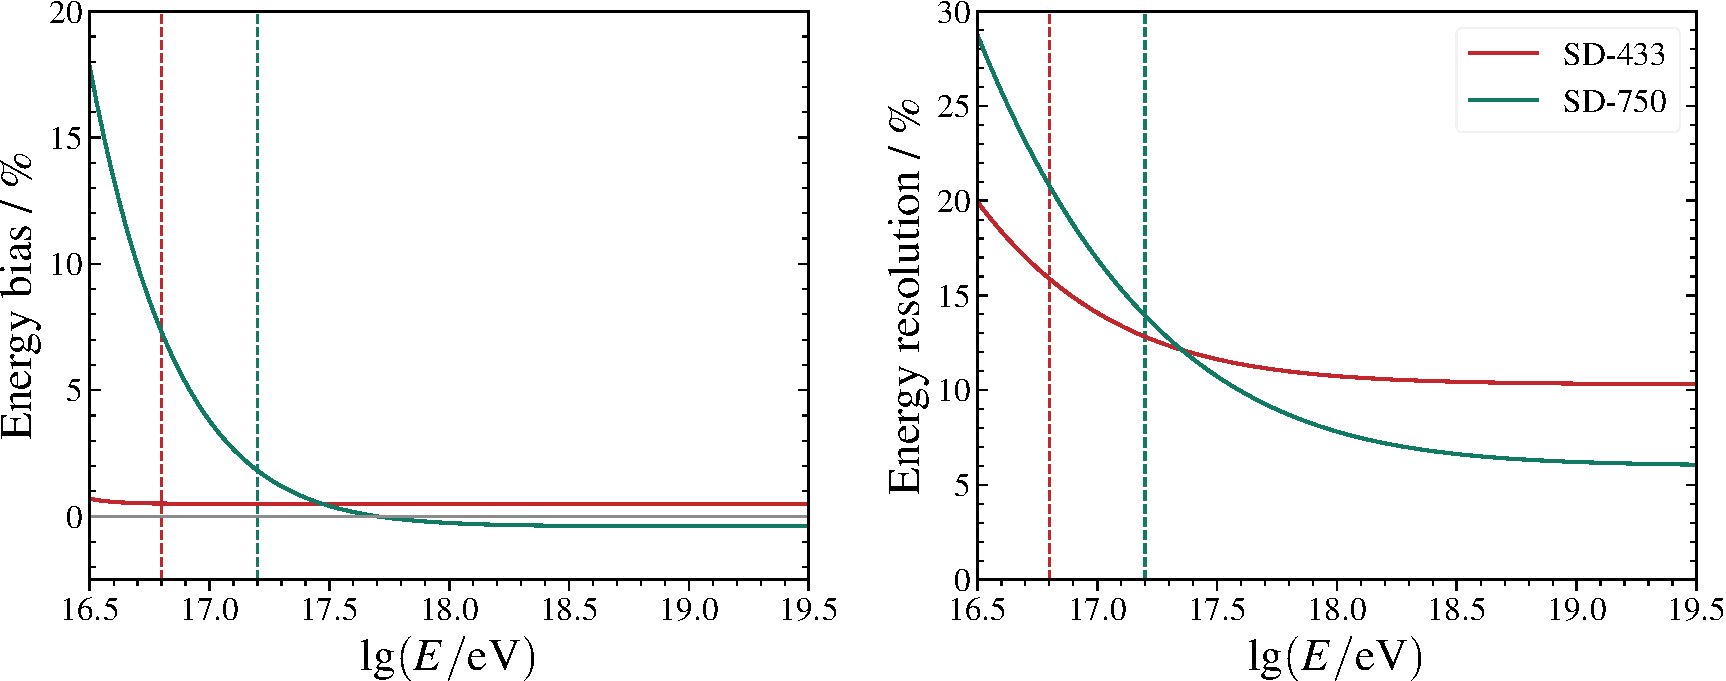
\includegraphics[width=\linewidth]{figures/chapter_combined/sd433_sd750_bias_resolution.pdf}
    \caption{Relative energy bias (left) and energy resolution (right) used to construct the \sd{433} and \sd{750} response matrices. The vertical dashed lines indicate the full-efficiency thresholds adopted for the two arrays.}
    \label{fig:sd433_sd750_response}
\end{figure}

With the efficiency from the previous section, the \sd{750} migration matrix can be constructed with the same formalism from \cref{sec:unfolded_spectrum}.
For this, the approximated matrix with the finer binning in $\Delta E_\text{true}=0.01$ is constructed with \cref{eq:matrix_approx} to make the matrix independent of the spectrum model.
The resulting migration matrix is presented in \cref{fig:sd750_migration_matrix}.
The dashed vertical line indicates the full efficiency threshold of the \sd{750} and the white diagonal line indicates $E_\text{true}=E_\text{recon}$.
As with the \sd{433}, the matrix is constructed for an energy range wider than the spectrum in order to avoid border effects from the neighbouring bin contributions.
Given that the resolution near the \sd{750} is similar to the one of the \sd{433}, the width of the spread in these rows is similar.
However, when comparing with \cref{fig:migration_matrix}, at higher energies, the spread around $E_\text{true}=E_\text{recon}$ is tighter due to the better resolution of the \sd{433}.
With this, using the raw spectrum, the forward folding fit can be performed.
\begin{figure}
    \centering
    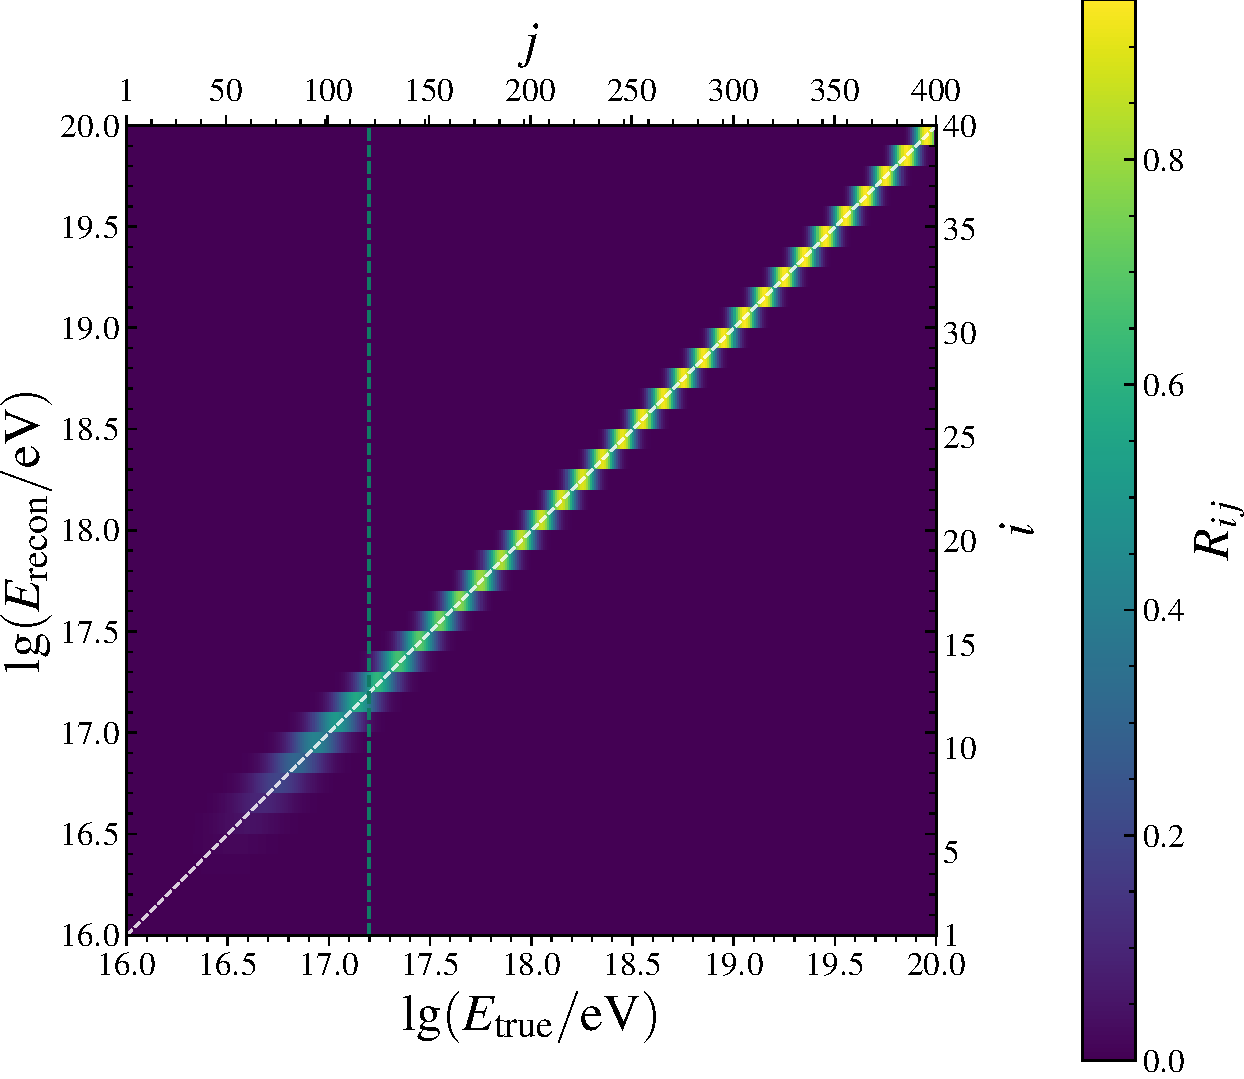
\includegraphics[width=0.78\linewidth]{figures/chapter_combined/sd750_migration_matrix.pdf}
    \caption{Migration matrix used for the updated \sd{750} spectrum. The horizontal axis gives the true-energy bin $j$ and the vertical axis the reconstructed-energy bin $i$; the additional axes give the corresponding logarithmic energies. The matrix includes the measured reconstruction efficiency, energy bias, and energy resolution.}
    \label{fig:sd750_migration_matrix}
\end{figure}

\subsection{Updated SD-750 spectrum}
\label{sec:sd750_spectrum}

The \sd{750} traditionally uses the Herald reconstruction.
For the updated and combined spectrum an update with the ICRC 2025 energy scale was performed as mentioned in the \cref{sec:calibration}.
However, the change in energy is minor with an energy difference less than $0.5\%$ around full efficiency and below $2\%$ at the highest energies.
This change in the energy scale leads to an intrinsic change in the spectrum, however minor.
The left panel of \cref{fig:sd750_raw_spectrum} shows the \sd{750} raw spectrum estimated with the updated dataset for $\theta<40^\circ$ together with the published in EPJC 2021.
The main difference is around $5\%$ at all energy range, due to a bug found in the code where the spectrum used included the bad periods.
This difference is constant in energy and can be seen amplified in the right panel of \cref{fig:sd750_raw_spectrum}.
The change in the energy explains the dependence in energy of the raw flux, that increases as the energy increases.
However, beyond the normalization, parameters compatible with the EPJC 2021 paper are found when using the same fit conditions, as can be seen in \cref{appendix:chapter_combined}.
The updated dataset was used for the \sd{433} calibration.

\begin{figure}
    \centering
    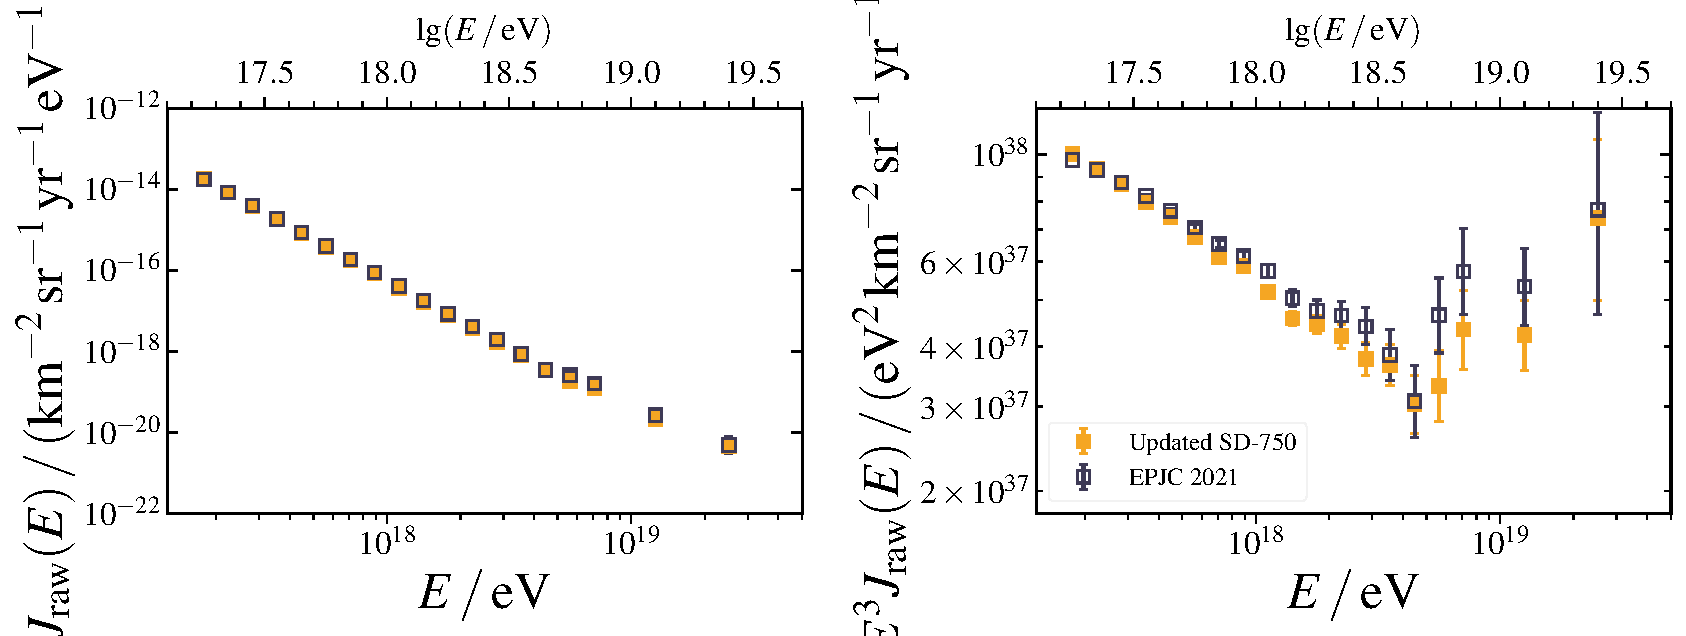
\includegraphics[width=0.9\linewidth]{figures/chapter_combined/sd750_raw_spectrum.pdf}
    \caption{Raw cosmic-ray spectrum measured with the updated \sd{750} dataset, compared with the spectrum reported in \cite{PierreAuger:2021:InfillSpectrum}. The left panel shows the differential flux and the right panel the flux multiplied by $E^3$. Both measurements are displayed using the same energy bins. Only statistical uncertainties are shown.}
    \label{fig:sd750_raw_spectrum}
\end{figure}

To fit the spectrum, the forward folding using the matrix from \cref{fig:sd750_migration_matrix} was used.
The higher energy range of the \sd{750} given its larger surface allows to include in the fit the next spectrum feature, the ankle.
This feature is a sharp hardening of the spectrum observed at around $4\,\mathrm{PeV}$. %Citation needed
To model the flux, an extension of \cref{eq:bplwst} was used,
\begin{align}
    J(E)=J_0
    \left(
    \frac{E}{10^{17}\,\mathrm{eV}}
    \right)^{\gamma_0
    }
    \prod \limits_{i=0}^{1}
    \left[
    1+
        \left(
        \frac{E}{E_{ij}}
        \right)
        ^{\frac{1}{\omega_{ij}}}
    \right]^{(\gamma_i-\gamma_j)\omega_{ij}},
    \label{eq:extended_bplwst}
\end{align}
\noindent where $j=i+1$.
The parameter $E_{12}$ describes the energy of the ankle, $\gamma_2$ is the spectral index after and $\omega_{12}$ is the parameter that governs the transition.
Given the sharpness of this feature, the transition parameter $\omega_{12}$ is fixed to 0.05 during the fit.

When the fit was performed, the second knee energy was fixed to the \sd{433} value during the fit, given that the full efficiency threshold of the \sd{750} did not allow to constrain all fit the parameters.
Nevertheless, when releasing it, $\lg(E_{01}/\mathrm{eV})=17.44\pm0.16$, very similar to the one obtained from the \sd{433} fit.
\cref{fig:sd750_unfolded_spectrum} shows the unfolded \sd{750} spectrum together with the fit.
The resulting fit parameters are shown in \cref{tab:sd750_fit_parameters}.
The obtained$\gamma_1$ slope after the second knee is compatible with the measurement from EPJC 2021 and the \sd{433} measurement from the previous chapter.
The ankle energy and slope are also compatible although the $\gamma_2$ is loosely constrained due to the lack of statistics of this array in this energy region.
The resulting deviance is $D^2=18.07$ for 17 degrees of freedom, corresponding to a $p$-value of $0.385$.

\begin{figure}
    \centering
    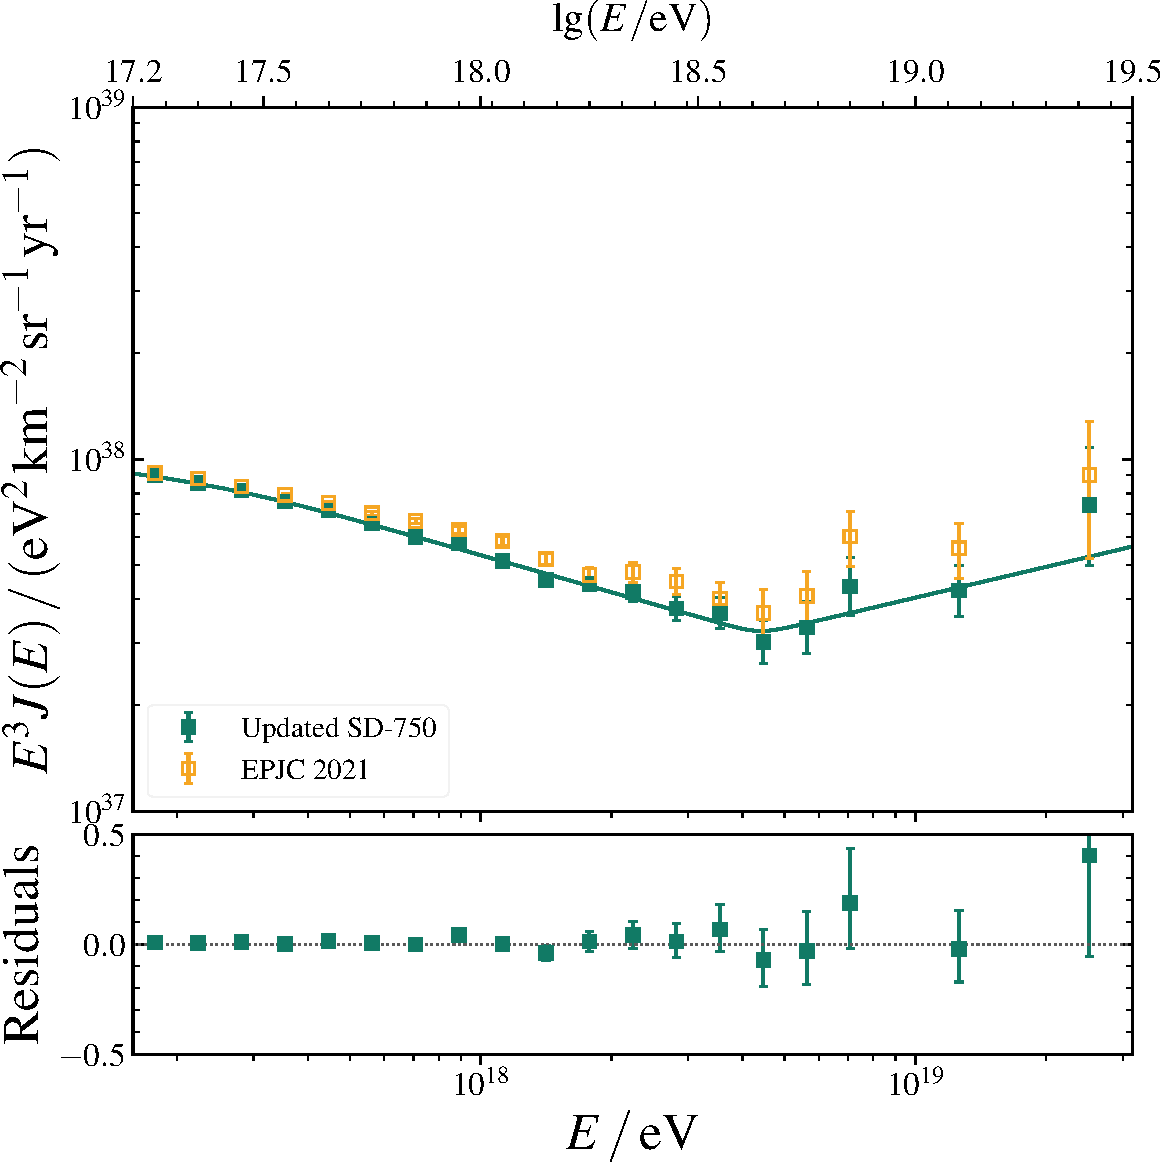
\includegraphics[width=0.82\linewidth]{figures/chapter_combined/sd750_unfolded_spectrum.pdf}
    \caption{Unfolded cosmic-ray spectrum measured with the updated \sd{750} dataset and its best-fit spectral model, obtained for $\lg(E/\mathrm{eV})\geq17.2$ with the second-knee position fixed to the \sd{433} result. The open squares show the unfolded spectrum reported in \cite{PierreAuger:2021:InfillSpectrum} for comparison. The lower panel shows the residuals of the updated \sd{750} points with respect to the fitted model; the published points are not included in the residuals. Only statistical uncertainties are shown.}
    \label{fig:sd750_unfolded_spectrum}
\end{figure}

\begin{table}
    \centering
    \caption{Parameters of the \sd{750} spectrum fit for $\lg(E/\mathrm{eV})\geq17.2$. The second-knee position $E_{01}$ is fixed to the \sd{433} result and the ankle width $\omega_{12}$ is fixed to $0.05$. The quoted uncertainties are statistical.}
    \label{tab:sd750_fit_parameters}
    \begin{tabular}{lcc}
        \toprule
        Parameter & Value\\
        \midrule
        $J_0\,/\,(10^{-13}\,\mathrm{km}^{-2}\,\mathrm{sr}^{-1}\,\mathrm{yr}^{-1}\,\mathrm{eV}^{-1})$ & $0.9861\pm0.0083$\\
        $\lg(E_{01}/\mathrm{eV})$ & $17.4401$ (fixed)\\
        $\omega_{01}$ & $0.264\pm0.159$\\
        $\gamma_0$ & $3.158\pm0.030$\\
        $\gamma_1$ & $3.351\pm0.024$\\
        $\lg(E_{12}/\mathrm{eV})$ & $18.641\pm0.085$\\
        $\omega_{12}$ & $0.05$\\
        $\gamma_2$ & $2.709\pm0.178$\\
        \bottomrule
    \end{tabular}
\end{table}

\section{Combined SD-433 and SD-750 spectrum}
\label{sec:combined_spectrum}

\begin{figure}
    \centering
    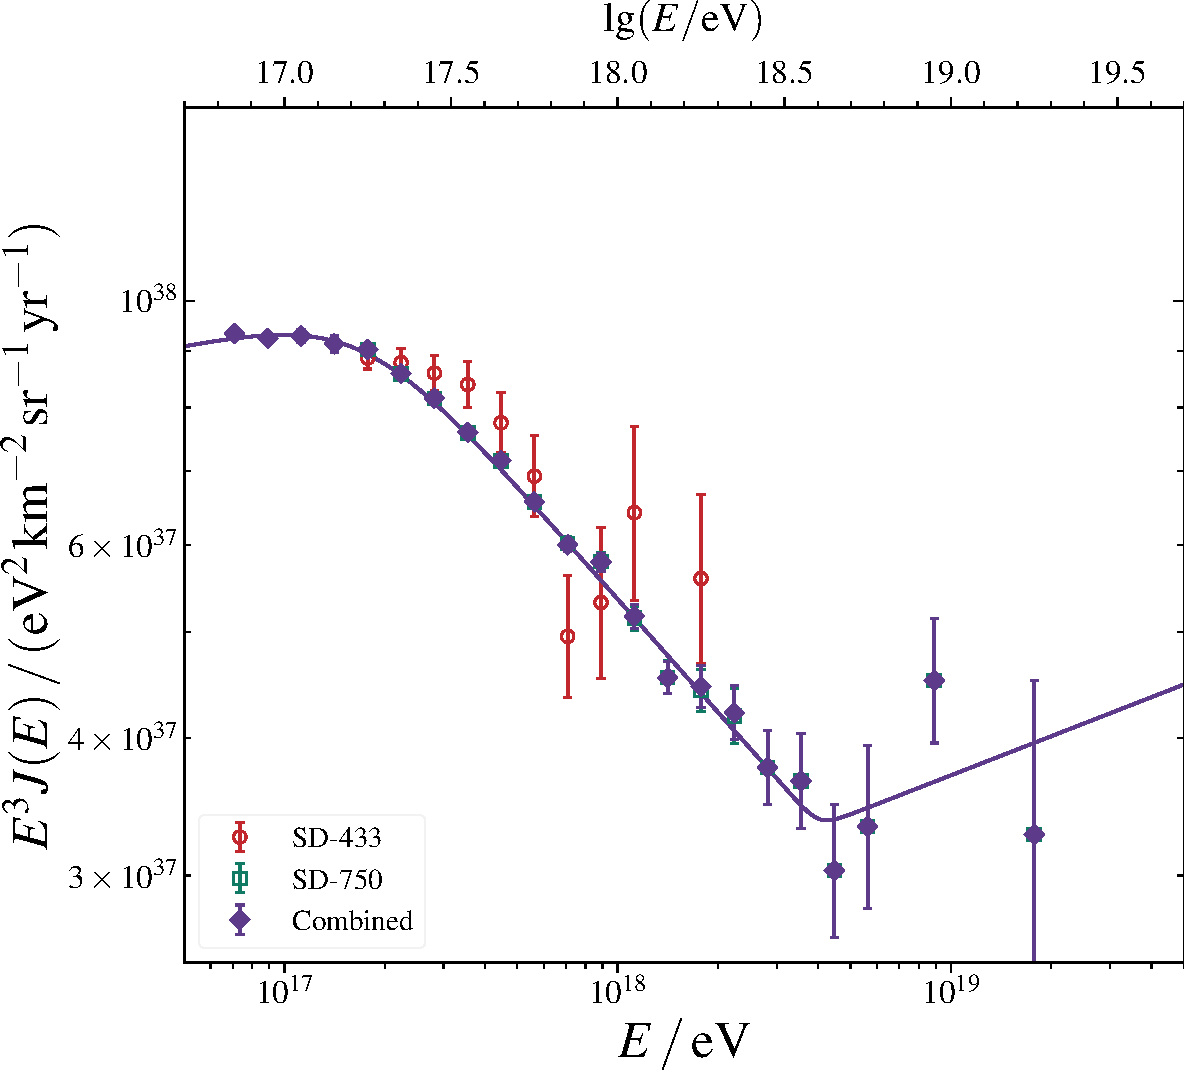
\includegraphics[width=0.82\linewidth]{figures/chapter_combined/sd433_sd750_combined_spectrum.pdf}
    \caption{Unfolded spectra measured with the \sd{433} and \sd{750}, together with the combined spectrum and common best-fit model. The combined spectrum uses the \sd{433} binning below $\lg(E/\mathrm{eV})=17.2$ and the \sd{750} binning at higher energies. Only statistical uncertainties are shown.}
    \label{fig:sd433_sd750_combined_spectrum}
\end{figure}

\begin{figure}
    \centering
    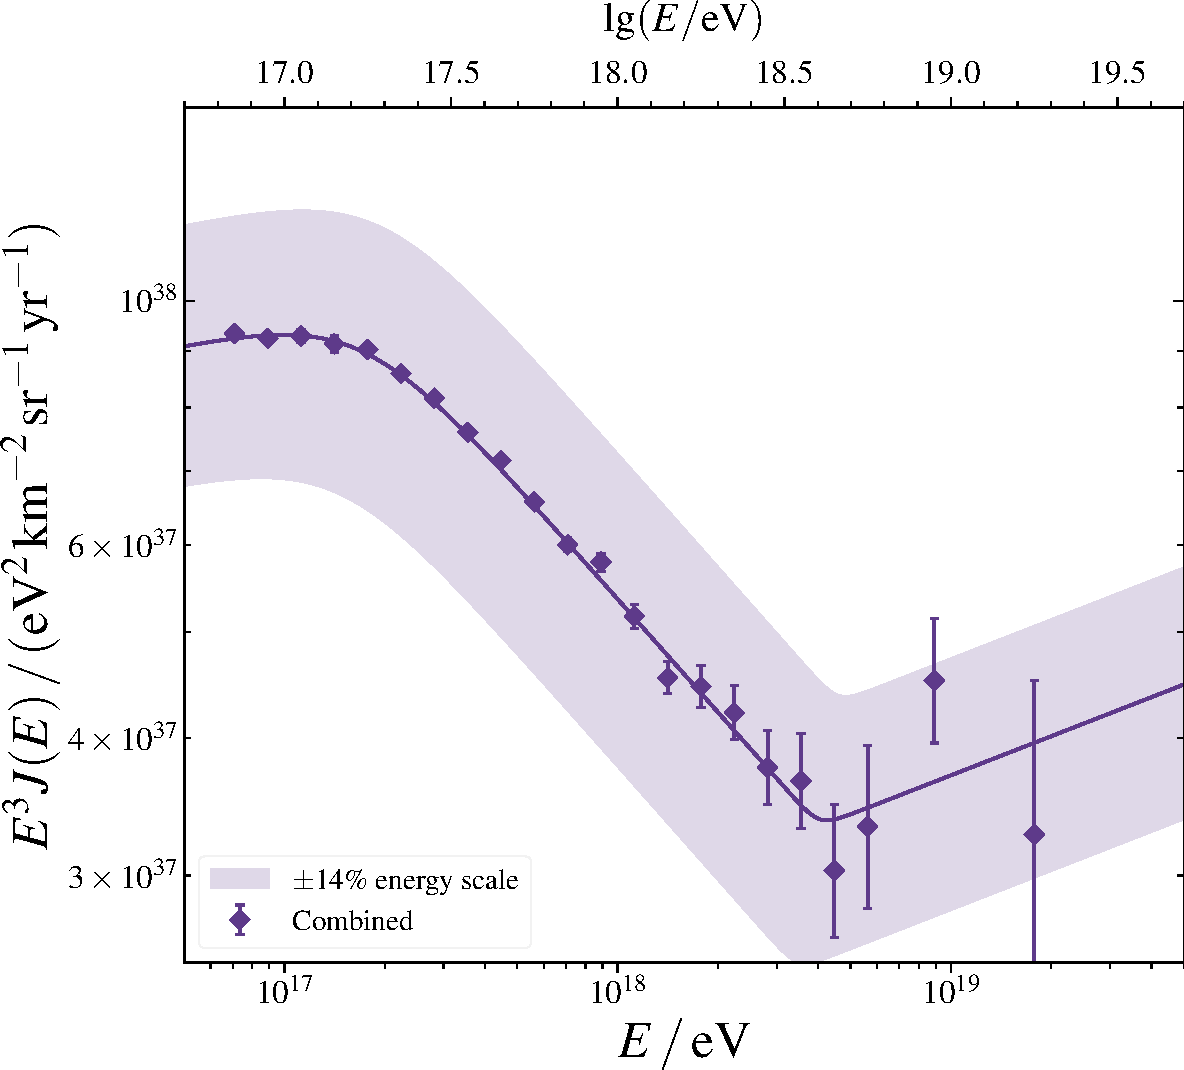
\includegraphics[width=0.82\linewidth]{figures/chapter_combined/sd433_sd750_combined_spectrum_systematic.pdf}
    \caption{Combined \sd{433}--\sd{750} spectrum and common best-fit model. The shaded region shows the effect of the $\pm14\%$ energy-scale uncertainty propagated through the fitted spectrum using \cref{eq:energy_systematic_bplwst}. The error bars represent statistical uncertainties.}
    \label{fig:sd433_sd750_combined_systematic}
\end{figure}

\section{Stability of the combined fit}

\begin{figure}
    \centering
    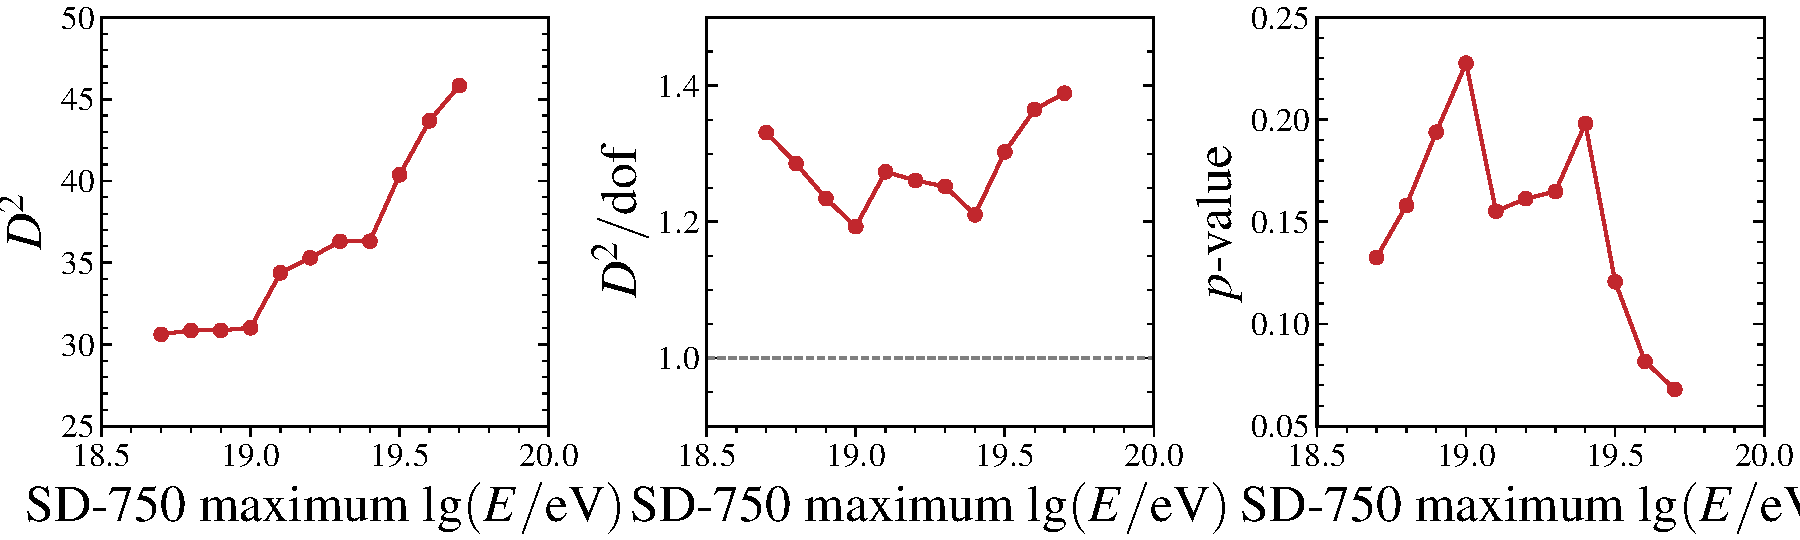
\includegraphics[width=\linewidth]{figures/chapter_combined/combined_fit_max_scan_deviance.pdf}
    \caption{Dependence of the combined-fit Poisson deviance, deviance per degree of freedom, and $p$-value on the maximum \sd{750} energy included in the fit. The \sd{750} lower boundary is fixed at $\lg(E/\mathrm{eV})=17.2$ and the \sd{433} fit range is kept unchanged.}
    \label{fig:combined_fit_max_scan}
\end{figure}

\begin{figure}
    \centering
    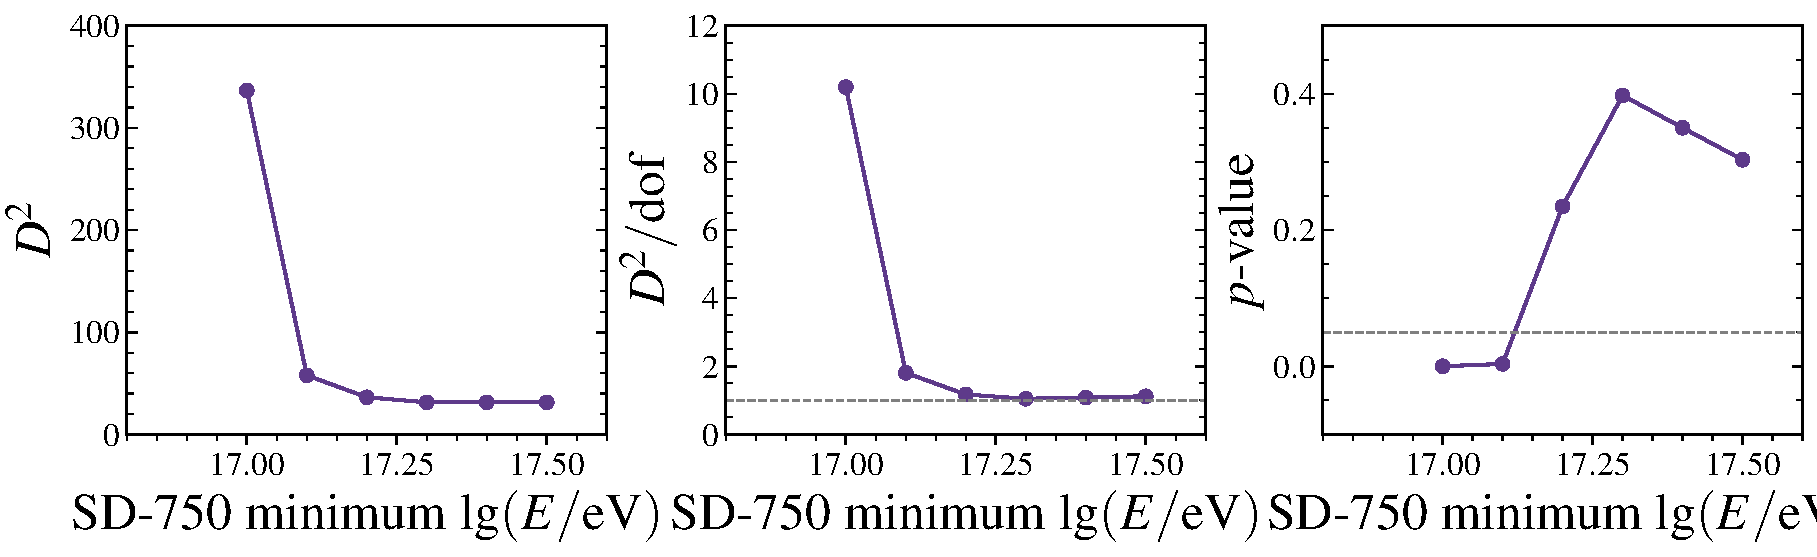
\includegraphics[width=\linewidth]{figures/chapter_combined/combined_fit_min_scan_deviance.pdf}
    \caption{Dependence of the combined-fit Poisson deviance, deviance per degree of freedom, and $p$-value on the minimum \sd{750} energy included in the fit. The scan covers $17.0\leq\lg(E_{\min}/\mathrm{eV})\leq17.5$; the fit first becomes acceptable at $\lg(E_{\min}/\mathrm{eV})=17.2$. The \sd{750} upper boundary is fixed at $\lg(E/\mathrm{eV})=19.4$, the \sd{433} fit range is unchanged, and the \sd{433} exposure is fixed to the value preferred by the nominal combined fit.}
    \label{fig:combined_fit_min_scan}
\end{figure}

\begin{figure}
    \centering
    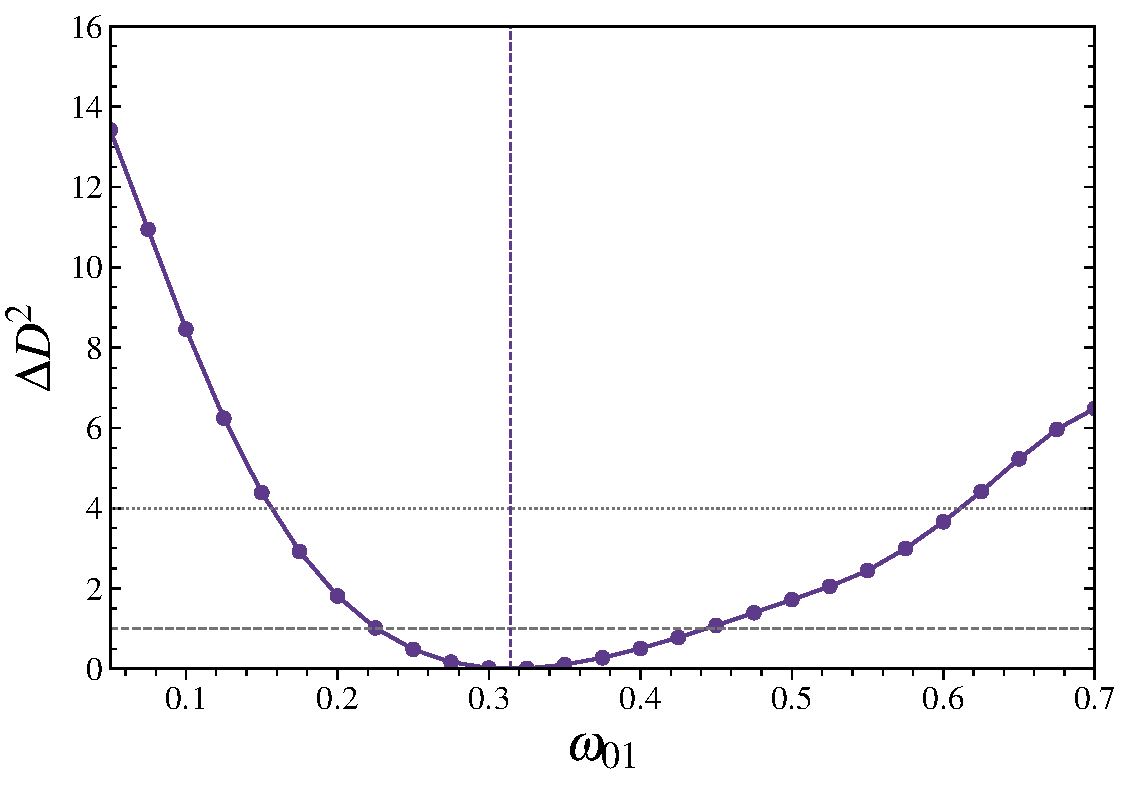
\includegraphics[width=0.8\linewidth]{figures/chapter_combined/combined_omega_profile.pdf}
    \caption{Profile of the combined-fit Poisson deviance as a function of the second-knee transition width $\omega_{01}$. At each fixed value of $\omega_{01}$, the remaining spectral parameters are profiled, while the \sd{433} exposure is fixed to the value preferred by the nominal combined fit and the calibration parameters are left unchanged. The horizontal lines indicate $\Delta D^2=1$ and $4$, and the vertical dashed line marks the best-fit value $\omega_{01}=0.314$.}
    \label{fig:combined_omega_profile}
\end{figure}

\end{document}
